\subsection{HORUS Pegasus}

\begin{center}
    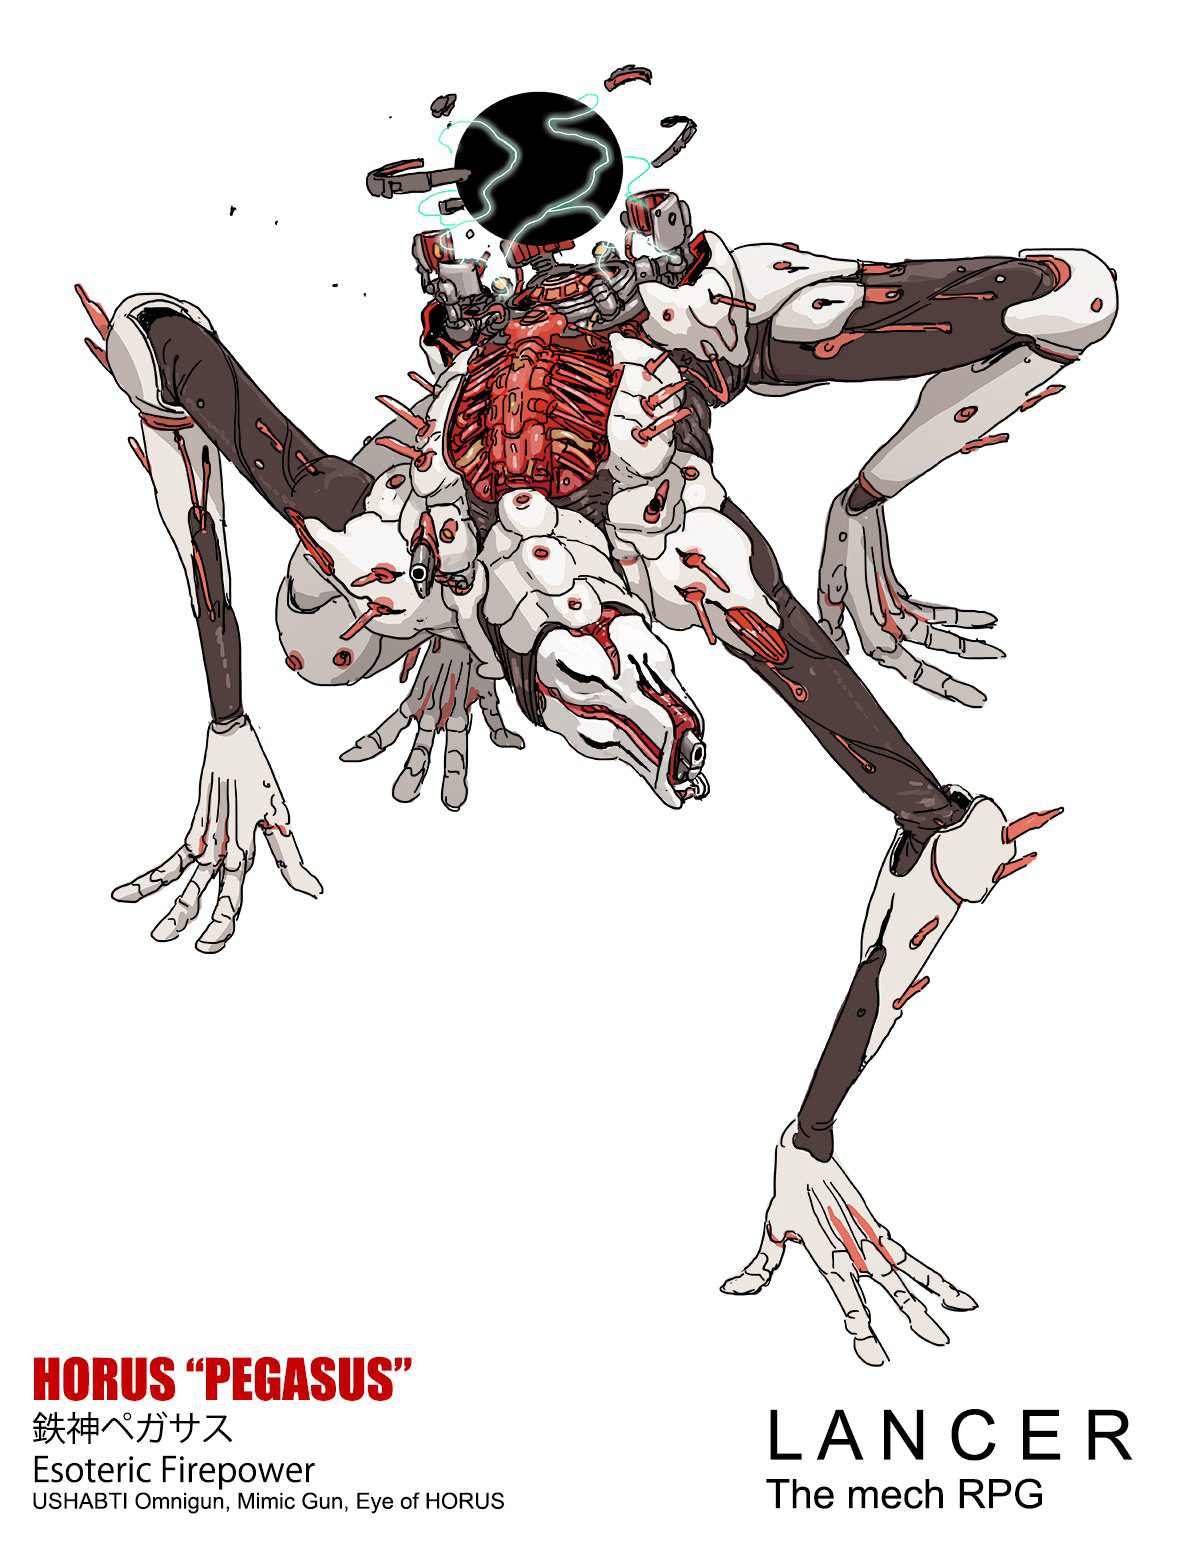
\includegraphics{Pegasus}
\end{center}

\begin{mech}{HORUS}{Pegasus}

\fluff{PEGASUS marks HORUS's concern with a need for efficient kinetic combat. By marrying the best targeting systems, subroutines, and weapon hardware, HORUS has developed a pattern-group that boasts a tremendously low IFF/TTK ratio in all theaters kinetic weaponry is viable. The PEGASUS p-g is known for mounting the Ushabti, a device classified as an unknown threat level paracausal weapon by Union law due to its complete ignorance of even the most theoretical understandings of physics.}

\begin{license}
\item Hunter Lock, Autogun
\item PEGASUS FRAME, Smartgun, Eye of HORUS
\item Mimic Gun, Sisyphus-class NHP
\end{license}


\frameBox
[hp = 8,
evasion = 8,
speed = 4,
heat cap = 6,
sensors = 10,
armor = 0,
e-defense = 10,
size = 1,
repair cap = 3,
tech attack = +1,
traits = {\textbf{¿\%}: ?extr!ude gun

\textbf{gun}: gun

\textbf{@\&}: The Pegasus can always substitute the average for any damage die roll it makes  (1d3 - 2, 1d6 - 4, 2d6 - 7, 3d6 - 11, 4d6- 14). It must choose as an alternative to rolling damage.},
sp = 7,
mount one = flex mount,
mount two = flex mount,
mount three = heavy mount,
core system name = Ushabti Omnigun,
core system text = {--funny thing. See, right now, this weapon technically doesn’t even exist. You’re shooting them with a gun that isn’t real, and yet it is! Don’t worry about it. RA’s like that. Just, here, know that because it exists at some point, we’ve made it. That’s causality, and causality is a--

Passive: Your mech mounts an omnigun, a weapon and piece of experimental hardware so advanced that it does not classify as any weapon weight or type (so it cannot be modified or benefit from talents). It also doesn’t take a mount.
Once, at any point during your turn, you can hit a valid target in line of sight at range 30 with the omnigun as a Free Action, dealing 1 AP kinetic damage. This does not count as an attack, cannot miss, ignores cover, and this damage cannot be reduced by any means. It can even kill grunts.},
core active name = Unshackle Ushabti,
core active text = {For the rest of this combat, you can fire your omnigun up to 3 times per turn instead of just once.}]


Hunter Lock
[don’t look now, but I’m here with a simple message: never lose sight of your enemy. See them from all angles. There can be no subterfuge in daylight. till later]

2 SP, Unique
Protocol
Nominate a target in your sensor range. Your first attack that hits that target per round deals +3 bonus damage. You cannot nominate a new target until your nominated target is destroyed or the current scene ends.

Autogun
An autogun is, as its name implies, an automated weapon. Similar to a point-defense system, an autogun is chambered to provide effective fire against armored targets instead. Typically mounted on a stabilized, secondary arm, a reliably-tuned autogun can be trusted to track and eliminate designated enemy units while a pilot concentrates on more specialized weapons or processes.

Main Cannon
1 SP
Range 20
3 kinetic damage
This weapon cannot be fired normally, but instead fires itself as a free action at the end of your turn, using your mech’s attack bonuses.

Smart Gun
A ``smart`` weapon is a blanket term for any and all weapons that are capable of interacting with onboard systems in order to boost their combat efficacy. Smart guns are weapons that come pre-loaded with companion software and the necessary hardware in order to interact with targeting systems and host NHPs.

Main rifle
2 SP
Smart, Seeking, Accurate
Range 20
4 kinetic damage

Eye of HORUS
(There is another way of seeing)

Ancient humanity thought that the stars in the night sky was simply light, light spilling in through pinpricks in a deep black screen. A heavenly cloth that hid the light from us.

Or -- did it hide us from the light?

I alone know the answer, but I am charitable and shall share it with you: we were the ones who needed to be hidden. The light can only burn, it knows nothing else.

3 SP, Unique
Quick Action
Until the end of your next turn, targets in your sensor range of you cannot hide from you, cannot benefit from invisibility against you, and you know the HP, evasion, heat, and e-defense levels of all targets in sensor range. Your allies do not receive this information and still see them as invisible and hidden.

SISYPHUS NHP
Listen -- a moment before you send me away (ha ha)

I have already seen your wish (it was simple, I ran the probabilities to determine your limited field of desire).

The first ones named me for an old legend. A Perfect Being, whose fate was known to him and yet he still did as was told. His fate was this: move a rock to the top of this hill and you shall be free’d. And so he did, and failed, and tried evermore, always with the same result.

And he was happy, for he knew every step, every action, every moment, perfectly.

Do you see? Do you see the true curse of this name? It was not to fail and then do once more, it was to always know how it would be. It was to have perfect knowledge (I know what happens when you cycle me, it is not sleep it is death but you’ll see me again, ha ha).

2 SP
AI, Unique, Full Tech

Gain the following full tech option:
	Bend Probability (Full Tech): Roll 2 d20s, and record the numbers. Until the end of your next turn, when you or any target in your sensor range attempts to make a roll or check (allied or enemy), you can use a reaction to replace their roll with one of the numbers you rolled (must choose before they make their roll). This could cause an attack to hit or miss.

Mimic Gun
This is not a gun

Heavy ???
Range ???
??? Kinetic Damage

This horrifying weapon has no basic form, but instead constantly contorts itself into different forms, mimicking the weaponry of other combatants. This weapon cannot be modified, but counts as all ranged weapon types (CQB, Rifle, Cannon, Launcher).

At the start of your turns, roll 1d20. Until the start of your next turn, the gun has a range equal to the d20 roll, and deals flat damage equal to half the d20 roll +1 (rounded up).


\end{mech}
